\documentclass {CSEThesis}
% Standard packages
\usepackage{amsmath}        % Extra math definitions
\usepackage{graphics}       % PostScript figures
\usepackage{setspace}       % 1.5 spacing
%\usepackage{psfig,epsfig}
\usepackage{multicol}
\usepackage{subfigure}
\usepackage{hyperref}
\usepackage{epsfig,color}
% Custom packages
%\usepackage[first]{datestamp}   % Datestamp on first page of each chapter


\usepackage{color}
%===== page layout
% Define the side margins for a right-side page
%\insidemargin = 1.3in \outsidemargin = 0.9in
% Above margin is space above the header
% Below margin is space below footer
%\abovemargin = 1.5in \belowmargin = 0.05in


\btptitle = {Title of Your BTP} % { and } are needed around your name
\name = {Student Name}          % and other feilds. don't remove.
\rollno = {03010104}
\email = {id.iitg.ernet.in}
\guide = {Your guide name}


\begin{document}

\begin{titlepage}
\begin{center}
\textheight 15.5in \textwidth 12.5in {\large\sf  \textbf{\the\btptitle}}\\[12ex]
{\small{\textsl{ \textbf{A Project Report Submitted \\
in Partial Fulfillment of the Requirements \\
for the Degree of \\
[3ex]\small \bf Bachelor of Technology}}}}\\
[16ex] \emph{by}
\\[2ex]
{\sf \sf \textbf{\the\name}\\
             (\the\rollno)}\\[1ex]
\emph{under the guidance of}\\[2ex]
{\sf \bf \the\guide} \\[7ex]

\vspace{1.2in}

 \begin{figure}[!h]
\centering
 
\includegraphics[width=0.15\textwidth]{IITPkdFullLogoColor}
 \end{figure}



{\small\bf DEPARTMENT OF COMPUTER SCIENCE AND ENGINEERING}  \\[1ex]
%{\small \bf{INDIAN INSTITUTE OF TECHNOLOGY PALAKKAD}}
%\\[2ex]
%
%  {\color{red} \hrule height 0.5ex}
% \vskip 1ex
% May \the\year 
\end{center}
\end{titlepage}



\raggedbottom
\doublespacing
\pagenumbering{roman}
\chapter*{\centering \underline{CERTIFICATE}}
\vskip 2ex \emph{\quad This is to certify that the work contained
in this thesis entitled ``\textbf{\the\btptitle}'' 
is a bonafide work of \textbf{\the\name}
(\textbf{Roll No. \the\rollno}), carried out in the Department of
Computer Science and Engineering, Indian Institute of Technology
Palakkad under my supervision and that it has not been submitted
elsewhere for a degree.} \vskip 15ex

\begin{flushright}
	\textbf{Your mentors name}\\
	Assistant/Associate Professor \\
	Department of Computer Science \& Engineering \\
	Indian Institute of Technology Palakkad
\end{flushright}
\hfill 
\hfill 






\chapter*{\centering Acknowledgements}
\quad Apart from the efforts of myself, the success of any project depends largely on the encouragement and guidelines of many others.
I take this opportunity to express my gratitude to the people who have been instrumental in the successful completion of this project.
I would like to show my greatest appreciation to Dr. Chandra Shekar. I can’t say thank you enough for his tremendous support and help.
I feel motivated and encouraged every time I attend his meeting.
Without his encouragement and guidance, this project would not have materialized.

\tableofcontents 

\addcontentsline{toc}{chapter}{List of Figures} 
\listoffigures 

\addcontentsline{toc}{chapter}{List of Tables} 
\listoftables

\pagenumbering{arabic}
\def\headrulehook{\color{black}}      % Color the header rule

%========== Chapters
\typeout{}
\chapter{Introduction}
\label{ch:introduction}
\pagenumbering{arabic}\hspace{3mm}

This chapter discusses anomaly detection, its use cases and some major challenges.

\section{Anomaly Detection}
\label{sec:anomaly-detection-definition}

Anomaly detection (also outlier detection) is the identification of rare items, events or observations which raise suspicions by differing significantly from the majority of the data.
Typically, the anomalous items will translate to some kind of problem such as bank fraud, a structural defect, medical problems or errors in a text.
Anomalies also known as outliers, novelties, noise, deviations and exceptions.

Three broad categories of anomaly detection techniques exist:

\begin{enumerate}
    \item Unsupervised anomaly detection techniques detect anomalies in an unlabeled test data set under the assumption that the majority of the instances in the data set are normal by looking for instances that seem to fit least to the remainder of the data set.
    \item Supervised anomaly detection techniques require a data set that has been labeled as "normal" and "abnormal" and involves training a classifier (the key difference to many other statistical classification problems is the inherently unbalanced nature of outlier detection).
    \item Semi-supervised anomaly detection techniques construct a model representing normal behavior from a given normal training data set, and then test the likelihood of a test instance to be generated by the learnt model.
\end{enumerate}

We will restrict ourselves to unsupervised anomaly detection and semi-supervised anomaly detection problem.

\section{Use Cases}
\label{sec:anomaly-detection-use-cases}

The ability to detect anomalies has significant relevance, and anomalies often provides critical and actionable information in various application domains.

Identification of potential outliers is important for the following reasons: \cite{EngineeringStatsHandbook}

\begin{enumerate}
    \item An outlier may indicate bad data.
    For example, the data may have been coded incorrectly, or an experiment may not have been run correctly.
    If it can be determined that an outlying point is in fact erroneous, then the outlying value should be deleted from the analysis (or corrected if possible).
    \item In some cases, it may not be possible to determine if an outlying point is bad data.
    Outliers may be due to random variation or may indicate something scientifically interesting.
    In any event, we typically do not want to simply delete the outlying observation.
\end{enumerate}

For example, anomalies in credit card transactions could signify fraudulent use of credit cards.
An anomalous spot in an astronomy image could indicate the discovery of a new star.
An unusual computer network traffic pattern could stand for unauthorised access.
These applications demand anomaly detection algorithms with high detection accuracy and fast execution.

\section{Masking and Swamping}
\label{sec:masking-and-swamping-definition}

Masking and swamping is the biggest problem affecting any anomaly detection algorithm.

Masking is the existence of too many anomalies concealing their own presence.
It happens when anomaly clusters become large and dense.
For example, if we are testing for a single outlier when there are in fact more outliers, these additional outliers may influence the value of the test statistic enough so that no points are declared as outliers.

On the other hand, swamping refers to situations where normal instances are wrongly identifying as anomalies.
It happens when the number of normal instances increases, or they become more scattered.
For example, if we are testing for two or more outliers when there is in fact only a single outlier, both points may be declared outliers.

Masking is one reason that trying to apply a single outlier test sequentially can fail.
For example, if there are multiple outliers, masking may cause the outlier test for the first outlier to return a conclusion of no outliers.
So the testing is not performed for any additional outliers.

\section{Concept drift}
\label{sec:concept-drift-definition}

In the case of streaming data, the anomaly context can change over time.
For example, consider a user's behaviour change from one system to another.
The anomaly detection algorithm should adapt to this change in the behaviour of the external agent.
This deviation of the normal behaviour time to time is called concept drift.
Any online anomaly detection algorithm must have a way to deal with this.


\section{Organization of The Report}
\label{sec:organization-of-the-report}

This chapter [\ref{ch:introduction}] provides a background for the topics covered in this report.
We provided a description of anomaly detection problem and discussed some use cases.
Then we discussed some challenges to anomaly detection problem: masking, swamping and concept drift.
In the next chapter [\ref{ch:isolation-forest}] we will discuss a very efficient ensemble method Isolation Forest for anomaly detection.
In chapter [\ref{ch:pidforest}] we will discuss another ensemble method PIDForest which has been recently developed.
The major drawback of the above mentioned algorithms is that they are used in offline setting without dealing with concept drift.
Most of the anomaly detection algorithm is offline and fail to address the problem of concept drift.
In chapter [\ref{ch:contributions}] we will present some methods to address these issues.
In chapter [\ref{ch:ai-image-compression}] we will review our work did till mid-sem.
And finally in chapter [\ref{ch:conclusion-future-work}], we conclude with some future works.

\vspace{2em}

\textbf{Code Repository: } \url{https://github.com/KishoreKaushal/AnomalyDetection}

\textbf{Report Repository: } \url{https://github.com/KishoreKaushal/btp-report}

\cleardoublepage 
\typeout{}
\chapter{Isolation Forest}
\label{ch:isolation-forest}

\section{Isolation based anomaly detection}
\label{sec:isolation-based-anomaly-detection}

Isolation is the process or fact of isolating or being isolated.
The authors of \cite{10.1145/2133360.2133363} proposed an isolation based anomaly detection which takes advantage of two quantitative properties of anomalies:
\begin{enumerate}
    \item They are the minority consisting of few instances.
    \item They have attribute-values that are very different from those of normal instances.
\end{enumerate}

Hence, anomalies are 'few and different' which make them more susceptible to a mechanism we called Isolation.
Isolation can be implemented by any means that separates instances.
Lui et al. \cite{10.1145/2133360.2133363} proposed to use a binary tree structure called isolation tree (iTree) which can be constructed effectively to isolate instances.
Because of the susceptibility to isolation, anomalies are more likely to be isolated closer to the root of an iTree;
whereas normal points are more likely to be isolated at the deeper end of an iTree.

The proposed method, called Isolation Forest (iForest) builds an ensemble  builds an ensemble of iTrees for a given data set.
Anomalies are those instances which have short average path lengths on the iTrees.
There are two training parameters and one evaluation parameter in this method: the training parameters are the number of trees to build and subsampling size.
The evaluation parameter is the tree height limit during evaluation.

\vspace{1em}
\begin{figure}[!ht]
    \label{fig:isolating-a-point}
    \centering
    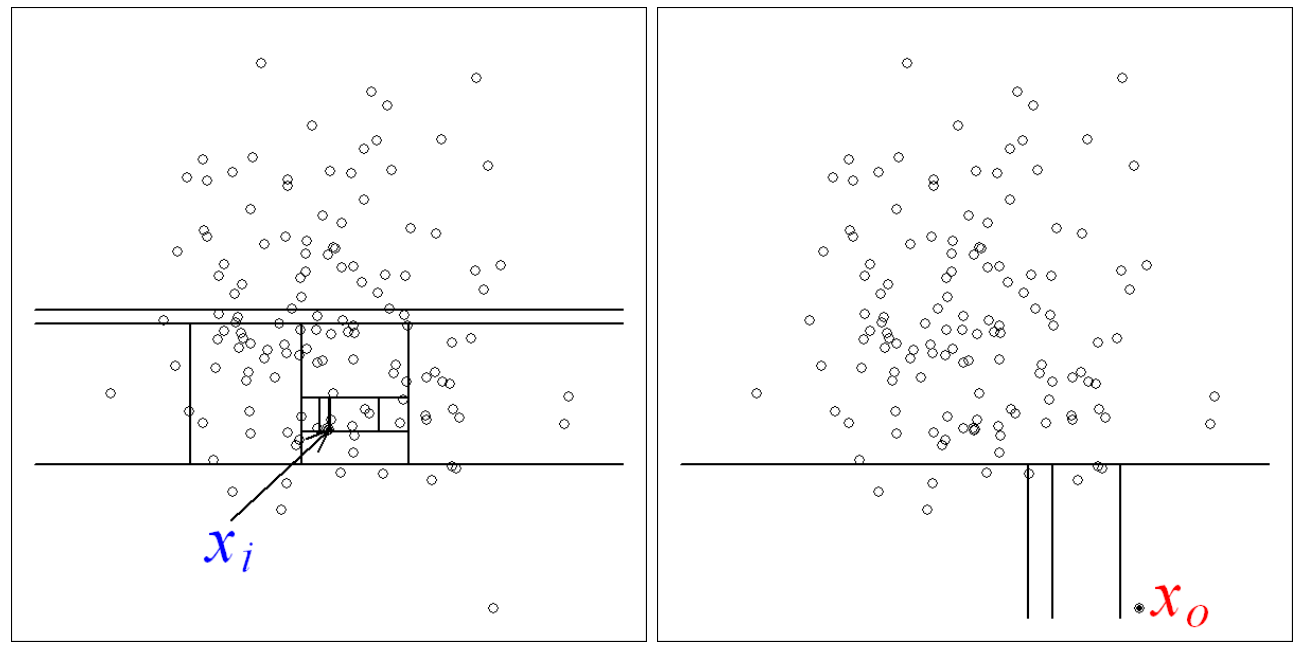
\includegraphics[width=0.80\textwidth]{../fig/chapter2/isolating-a-point.png}
    \captionsource{\textbf{Left}: a normal point $x_i$ requires twelve random partitions to be isolated; \textbf{Right}: an anomaly $x_o$ requires only four partitions to be isolated.}
    {Lui et al. \cite{10.1145/2133360.2133363}}
\end{figure}


\vspace{1em}
\begin{figure}[!ht]
    \label{fig:path-length}
    \centering
    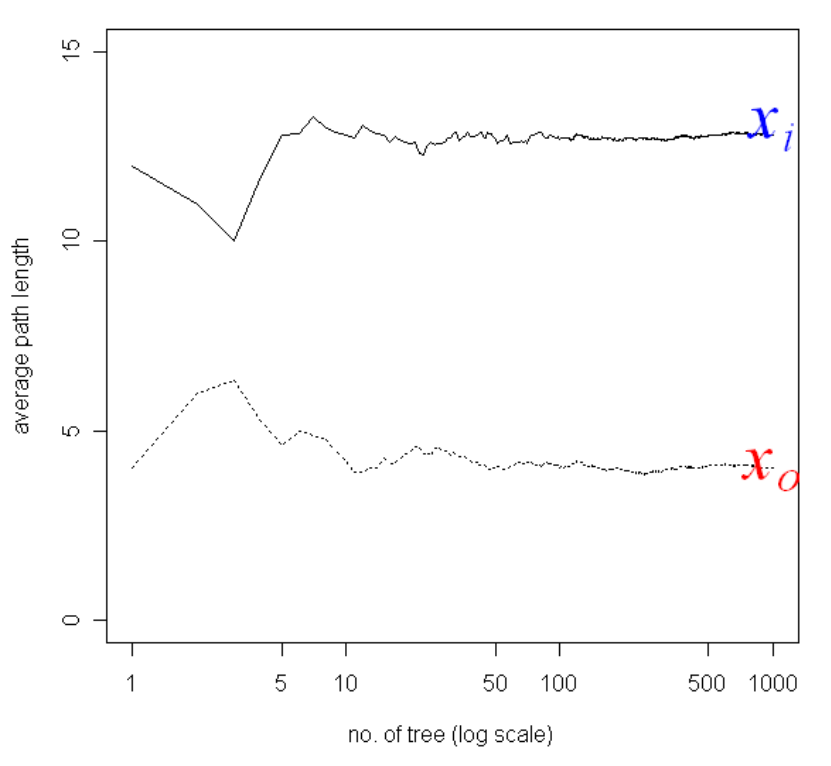
\includegraphics[width=0.50\textwidth]{../fig/chapter2/path-length-for-that-point.png}
    
    \captionsource{Averaged path lengths of $x_i$ and $x_o$ converge when the number of trees increases.}
    {Lui et al. \cite{10.1145/2133360.2133363}}
\end{figure}

\section{Training Stage}
\label{sec:iforest-training}

Formally, we can define isolation forest as follows:

\begin{defn}
    \label{defn:isolation-tree}
    (Isolation Tree)
    Let T be a node of an isolation tree.
    T is either an external-node with no child, or an internal-node with one test and exactly two daughter nodes $(T_l, T_r)$.
    A test at node $T$ consists of an attribute $q$ and a split value $p$ such that the test $q < p$ determines the traversal of a data point to either $T_l$ or $T_r$.
    Let X = $\{x_1, ..., x_n\}$ be the given data set of a d-variate distribution.
    A sample of instances X'$\subset$ X is used to build an isolation tree$^{[\ref{alg:iTree}]}$.
    We recursively divide X' by randomly selecting an attribute q and a split value p, until either: i) Node has only one instance ii) Or, all data at the node have the same values.
\end{defn}


\begin{defn}
    \label{defn:isolation-forest}
    (Isolation Forest)
    Isolation forest is defined as 4-tuple $(X, t, \psi, S)$ where
    \vspace{-1em}
    \begin{itemize}
        \setlength\itemsep{-1em}
        \item X is input data,
        \item t is number of trees,
        \item $\psi$ is subsampling size and
        \item S is the set of isolation trees.
    \end{itemize}
    \vspace{-1em}
    The elements of set S is constructed$^{[\ref{alg:iForest}]}$ by sampling $\psi$ instances from X without replacement.
\end{defn}

\vspace{1em}
\begin{algorithm}[H]
    \caption{$iForest(X,t,\psi)$}\label{alg:iForest}
    \setstretch{1.2}
    \SetAlgoLined
    \KwComplexity{Time - $O(t\psi^2)$, Space - $O(t\psi)$}
    \KwInput{$X$ - input data, $t$ - number of trees, $\psi$ - subsampling size}
    \KwOutput{List of $iTrees$}

    $Forest \: \leftarrow $ EmptyList

    \For {$i = 1$ to $t$}{
        $X' \: \leftarrow \: sampleWithoutReplacement(X,\psi)$

        $Forest.append(iTree(X'))$
    }

    \Return{Forest}
\end{algorithm}

\vspace{1em}
\begin{algorithm}[H]
    \caption{$iTree(X)$}\label{alg:iTree}
    \setstretch{1.2}
    \SetAlgoLined
    \KwComplexity{Time - $O(\psi^2)$, Space - $O(\psi)$}
    \KwInput{$X$ - input data}
    \KwOutput{an $iTree$}

    q $\leftarrow \: RandomChoice(X.attributes)$

    p $\leftarrow \: RandomNumber(X[$splitAttr$].min(), X[$splittAttr$].max())$

    tree $\leftarrow$ Node \{ left $\leftarrow$ None, right $\leftarrow$ None, size $\leftarrow \: X.size$

    \qquad\qquad\qquad splitAttr $\leftarrow$ q, splitVal $\leftarrow$ p\}

    \If{X.size $>$ 1 and X[splitAttr].numUnique() $>$ 1}{
        $X_{l} \: \leftarrow  \: X.where(q < p)$

        $X_{r} \: \leftarrow  \: X.where(q \geq p)$

        tree.left $\leftarrow \: iTree(X_{l})$

        tree.right $\leftarrow \: iTree(X_{r})$
    }

    \Return{tree}
\end{algorithm}
\vspace{1em}

\section{Evaluation Stage}
\label{sec:iforest-evaluation}


\vspace{1em}
\begin{algorithm}[H]
    \caption{$PathLength(x, T, hlim, e)$}\label{alg:PathLength}
    \DontPrintSemicolon
    \setstretch{1.2}
    \SetAlgoLined
    \KwComplexity{Time - $O(t\psi)$, Space - $O(1)$}
    \KwInput{$x$ - input instance, $T$ - an iTree, $hlim$ - height limit, $e$ - current path length to be initialized to zero when called first time}
    \KwOutput{path length of $x$}

    \If{ (T.right is None) and (T.left is none) and (e $\geq$ hlim)}{

        \Return $e + c(T.size)$ \tcp*{c(...) is defined in Equation \ref{eq:average-path-length-of-unsuccessful-searches-bst}}

    }

    $a \: \leftarrow \: T.splitAttr$

    \If{ $x[a] < T.splitVal$}{
        \Return  $PathLength(x, T.left, hlim, e + 1)$
    }
    \Else{
        \Return  $PathLength(x, T.right, hlim, e + 1)$
    }
\end{algorithm}
\pagebreak

In the evaluation stage$^{[\ref{alg:PathLength}]}$, a single path length $h(x)$ is derived by counting the number of edges $e$ from the root node to an external node as instance $x$ traverses through an iTree.
When the traversal reaches a predefined height limit $hlim$, the return value is $e$ plus an adjustment $c(size)$.
This adjustment accounts for estimating an average path length of a random sub-tree which could be constructed using data of $size$ beyond the tree height limit.
When $h(x)$ is obtained for each tree of the ensemble, an anomaly score is computed.
The anomaly score and the adjustment $c(size)$ is defined in the next section.

\section{Anomaly Score}
\label{sec:iforest-anomaly-score}

The difficulty in deriving an anomaly score from $h(x)$ is that while the maximum possible height of iTree grows in the order of $\psi$, the average height grows in the order of $log\,\psi$.
When required to visualize or compare path lengths from models of different subsampling sizes, normalization of $h(x)$ by any of the above terms either is not bounded or cannot be directly compared.
Thus, a normalized anomaly score is needed for the aforementioned purposes.

Since iTrees have an equivalent structure to Binary Search Tree, the estimation of average $h(x)$ for external node terminations is the same as that of the unsuccessful searches in BST.

Section 10.3.3 of \cite{10.5555/289373} gives the average path length of unsuccessful searches
in BST as:

\vspace{-2em}
\begin{equation}
    \label{eq:average-path-length-of-unsuccessful-searches-bst}
    \begin{split}
        c(\psi) =  \left\{
        \begin{matrix}
            2H(\psi -1) - 2(\psi -1)/n & \text{for}\: \psi>2,\\
            1 &  \text{for}\: \psi=2,\\
            0 & \text{otherwise.}
        \end{matrix}\right.
    \end{split}
\end{equation}

where $H(i) \approx \ln(i) + 0.5772156649$  (euler's constant), is the harmonic number. As $c(\psi)$ is the average of $h(x)$ given $\psi$, we use it to normalise $h(x)$.
The anomaly score $s$ of an instance $x$ is defined as:

\begin{equation}
    \label{eq:iforest-anomaly-score-for-an-instance}
    s(x,\psi) = 2^{\frac{-E[h(x)]}{c(\psi)}}
\end{equation}

where $E[h(x)]$ is the average of $h(x)$ from a collection of iTrees. 

Anomaly score $s(x,\psi)$ is interpreted as follows:

\begin{enumerate}
    \vspace{-1em}
    \setlength\itemsep{-1em}
    \item if $s \approx 1$, instance is abnormal
    \item if $s \approx 0$, instance is nominal
    \item if $s \approx 0.5$, no distinct anomaly
\end{enumerate}

\vspace{1em}
\begin{figure}[!ht]
    \centering
    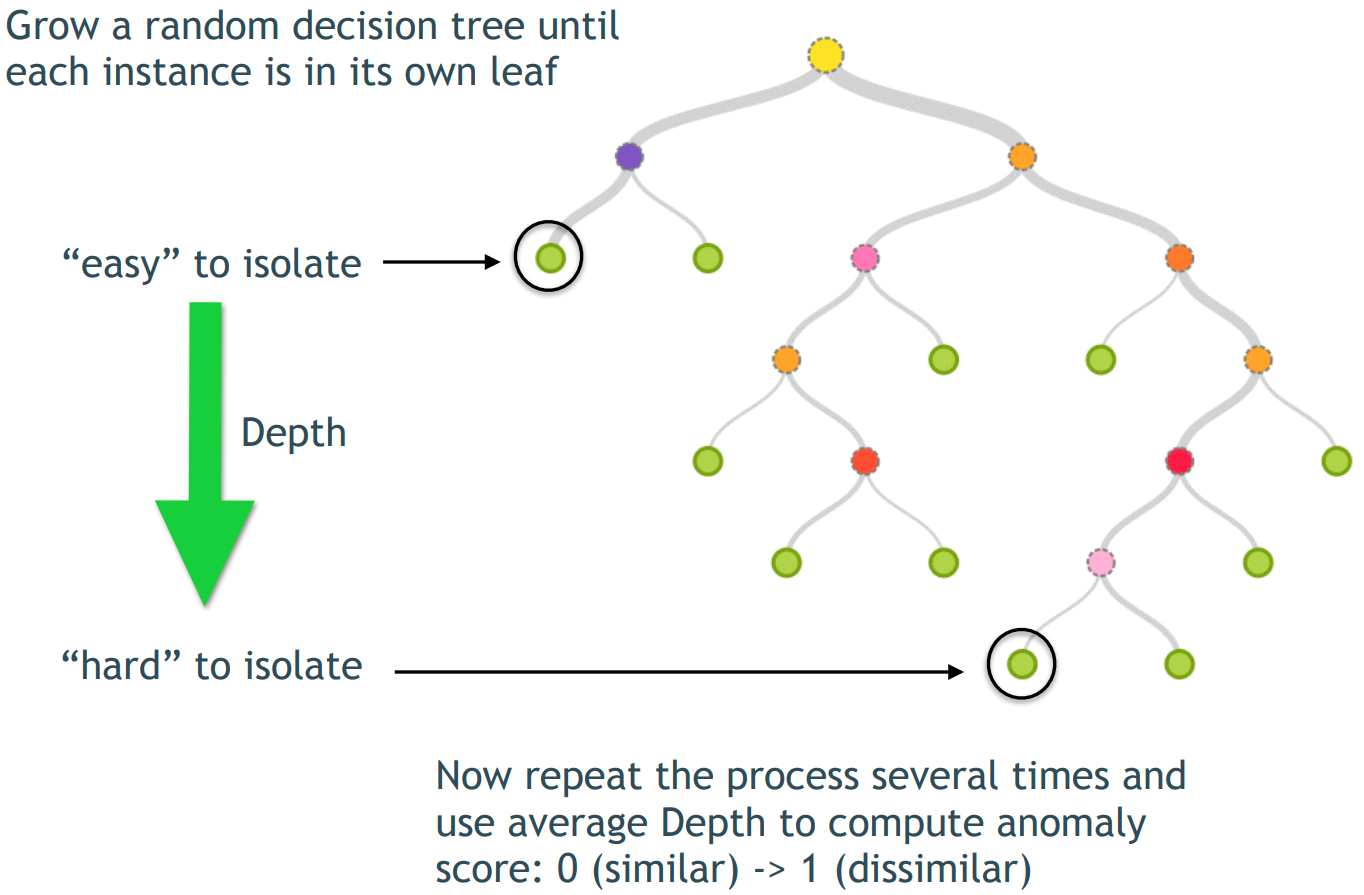
\includegraphics[width=0.80\textwidth]{../fig/chapter2/iforest-visualization.png}
    \captionsource{Isolation forest}
    {\href{https://www.slideshare.net/mlvlc/l14-anomaly-detection}{slideshare.com}}
    \label{fig:iforest-visualization}
\end{figure}

In practical use cases, one has to set a threshold deciding the result.
And finding a good threshold is a very difficult task.
Most of the times the anomalous points' score overlaps with the nominal points' score.

\section{Isolation vs. Distance and Density}
\label{sec:isolation-vs-distance-density}

Using basic density measures, the assumption is that ‘Normal points occur in dense regions, while anomalies occur in sparse regions’.
Using basic distance measures, the basic assumption is that ‘Normal point is close to its neighbours and anomaly is far from its neighbours’.

There are violations of these assumptions: i) high density and short distance do not always imply normal instances ii) low density and long distance do not always imply anomalies.

\begin{figure}
    \label{fig:high-density-short-distance}
    \centering
    \subfigure[density based method k-NN]{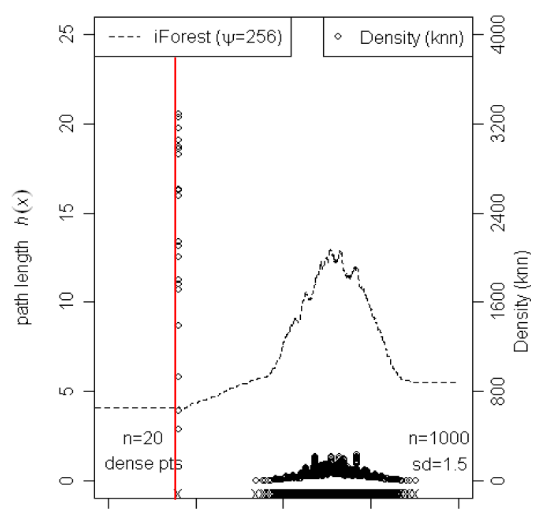
\includegraphics[width=0.4\textwidth]{../fig/chapter2/high-density-short-distances-1.png}}
    \subfigure[distance based method kth-distance]{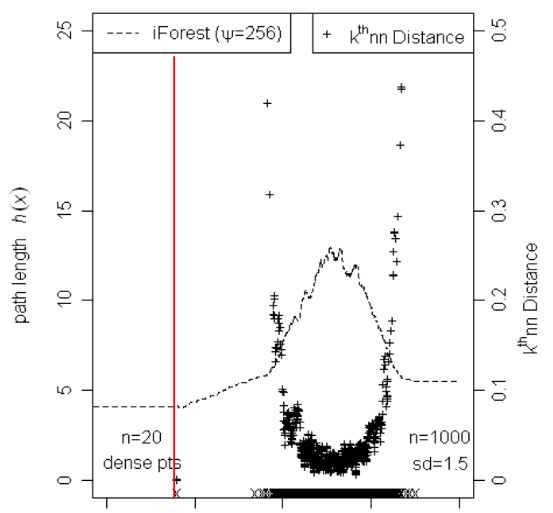
\includegraphics[width=0.4\textwidth]{../fig/chapter2/high-density-short-distances-2.png}}
    \captionsource{High density and short distance do not always imply normal instances.}
    {Lui et al. \cite{10.1145/2133360.2133363}}
\end{figure}

\begin{figure}
    \label{fig:low-density-long-distance}
    \centering
    \subfigure[density based method k-NN]{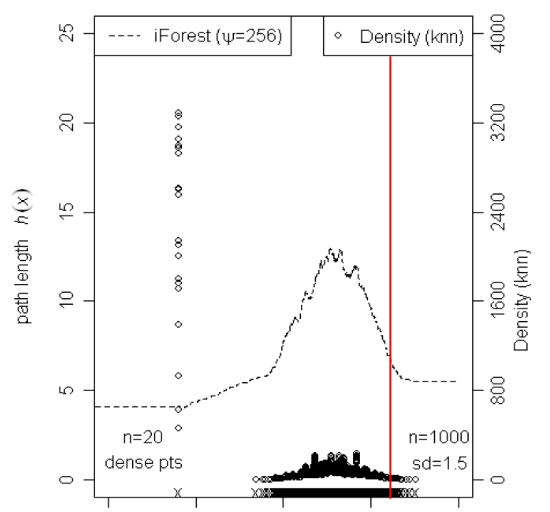
\includegraphics[width=0.4\textwidth]{../fig/chapter2/low-density-long-distances-1.png}}
    \subfigure[distance based method kth-distance]{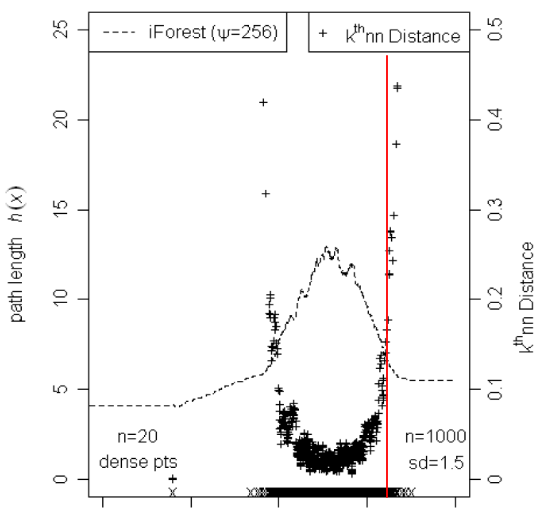
\includegraphics[width=0.4\textwidth]{../fig/chapter2/low-density-long-distances-2.png}}
    \captionsource{Low density and long distance do not always imply anomalies.}
    {Lui et al. \cite{10.1145/2133360.2133363}}
\end{figure}

Isolation forest compares favourably to distance and density  based methods in terms of accuracy and processing time.
Distance and density based suffers immensely in terms of accuracy and processing time because of curse of dimensionality.


Distance based methods also suffers from masking and swamping effect. 
In isolation forest, masking and swamping effects can be managed by adjusting the $hlim$ parameter during evaluation.
Refer section 4.5, 5.3 and 5.4 of Lui et al. \cite{10.1145/2133360.2133363}.


Codes for \href{https://github.com/KishoreKaushal/AnomalyDetection/blob/master/isolationforest/IsolationForest.py}{Isolation Forest} and \href{https://github.com/KishoreKaushal/AnomalyDetection/blob/master/isolationforest/IsolationTree.py}{Isolation Tree} can be found at \href{https://github.com/KishoreKaushal/AnomalyDetection}{this} repository.


\section{Conclusion}
\label{sec:iforest-conclusion}

To conclude, isolation forest is one of the most efficient and accurate methods for anomaly detection.
It outperforms various density and distance based methods like ORCA, DOLPHIN, LOF, ROF, etc and their variants in terms of accuracy and performance.
Still, there are some shortcomings of the isolation forest that we will discuss in next chapter.


\cleardoublepage 
\typeout{}
\chapter{PIDForest}
\label{ch:pidforest}

In \cref{ch:introduction} we discussed some challenges that an anomaly detection algorithm face.
In the previous chapter we discussed an isolation based ensemble method which is a very good method in terms of complexity and accuracy.
Isolation forest tried to address the problems related to masking and swamping.
In this chapter we will point out some major issues with isolation forest and discuss another ensemble method, which improves upon those issues.

\section{Issues with Isolation Forest}
\label{sec:issues-with-iforest}

\paragraph{Random Split:} iForest repeatedly samples a set $X'$ of $\psi$ points from $X$ and builds a random tree with those points as leaves. 
The tree is built by choosing a random co-ordinate $q$, and a random value $p$ in its range about which to split. 
Thus, isolation forest chooses which coordinate we split on as well as the breakpoint at random.
Hence, to be isolated at small depth frequently, picking splits at random must have a good chance of isolating an anomalous point.
Although, there are other variants like extended isolation forest which improves on this, but there are no significant improvements.

\paragraph{High Dimensionality:} As the number of co-ordinates or attributes increases, probability of choosing a sequence of attributes for split which gives rise to most of the anomalies will be very less. 
Hence, it is very likely that anomalous points won't be isolated near the root and false negative cases will increase. (In anomaly detection problems, anomaly is the true class.)

\paragraph{Presence of non-ordinal categorical attributes:} A very big limitation of isolation forest is that it only works for those datasets where all the features are real-values or ordinal. For example, consider a feature \textbf{HTTP\_REQUEST} which can take one of these values: \{GET, POST, DELETE, CONNECT, HEAD, TRACE, PUT, OPTIONS\}. We cannot use isolation forest on a dataset containing this feature because there is no way we can perform a comparison to split the data with this feature.

\section{Partial Identification}
\label{sec:partial-identification}

We will briefly discuss some concepts present in section 2 of Vatsal et al. \cite{NIPS2019_9710}. 

\paragraph{Notations:} Let $T$ denote a dataset of $n$ points in $d$ dimensions.
Given indices $S \subseteq [d]$ and $x \in R$, let $x_S$ denote the projection of $x$ onto coordinates in $S$.
All the logarithms are to base 2.

\subsection{Boolean Setting}
\label{subsec:boolean-setting}

In Boolean setting $T \subseteq \{0,1\}^d$ and assume that $T$ has no duplicates. 

\begin{defn}
    \label{defn:id-for-a-point}
    (ID for a point)
    \vspace{-1em}
    \begin{equation}
        \label{eq:ID}
        \begin{split}
        id = \{ S \mid S \subseteq [d], x \in T \textrm{ and } \forall y \in T \setminus x, \, x_S \neq y_S \}  \\
        ID(x,T) = arg \min_{S \subseteq [d]} \vert \{ S \mid S \subseteq [d], x \in T \textrm{ and } \forall y \in T \setminus x, \, x_S \neq y_S \} \vert
        \end{split}
    \end{equation}
    \vspace{-2em}
    \begin{equation}
        \label{eq:id-length}
        idLength(x,T) = \vert ID(x, T) \vert
    \end{equation}
\end{defn}

\begin{defn}
    \label{defn:impostor}
    (Impostor)
    \vspace{-1em}
    \begin{equation}
        \label{eq:impostor}
        Imp(x, T, S) = \{y \in T \mid x \in T, S \subseteq [d] \textrm{ and } x_S = y_S\}
    \end{equation}
\end{defn}


\begin{defn}
    \label{defn:partial-ids}
    (Partial ID) 
    \vspace{-1em}
    \begin{equation}
        \label{eq:PID}
        PID(x,T) = arg \min_{S \subseteq [d]} 
    (\vert S \vert + log_{2}(\vert Imp(x, T, S) \vert)),
    \end{equation}
    \vspace{-2em}
    \begin{equation}
        \label{eq:pidLength}
        pidLength(x,T) = \min_{S \subseteq [d]} 
    (\vert S \vert + log_{2}(\vert Imp(x, T, S) \vert)).
    \end{equation}
\end{defn}


\paragraph{Geometric view of pidLength:}
A subcube $C$ of $\{0, 1\}^d$ is the set of points obtained by fixing some subset $S \subseteq [d]$ coordinates to values in 0, 1. (Refer section 1 of \cite{ellis_2011})
The sparsity of $T$ in a subcube C is $\rho_{0,1}(T, C) = \frac{\vert C \vert}{\vert C \cap T\vert}$.
The notation $C \ni x$ means that $C$ contains $x$, hence $\min_{C \ni x}$ is the minimum over all $C$ that contain $x$.
Anomalies are points that lie in relatively sparse subcubes.
Low scores come with a natural witness: sparse subcube $PID(x, T)$ containing relatively few points from T\@.

\begin{defn}
    \label{defn:pidforest-anomaly-score}
    (Anomaly Score)
    \vspace{-1em}
    \begin{equation}
        \label{eq:pidforest-anomaly-score}
        s(x,T) = 2^{-pidLength(x,T)}
    \end{equation}
\end{defn}

\subsection{Continuous Setting}
\label{subsec:continuous-setting}

Without loss of generality assume that $T \subseteq [0,1]^d$.
Length of an interval $I = [a,b], 0 \leq a \leq b \leq 1$ is $len(I) = (b-a)$.
A subcube $C$ is specified by a subset of co-ordinates $S$ and intervals $I_j, \forall j \in S$.
It consists of all points such that $x_j \in I_j, \forall j \in S$.

\begin{defn}
    \label{defn:volume-of-subcube}
    (Volume of a Subcube)
    \vspace{-1em}
    \begin{equation}
        \label{eq:volume-of-subcube}
        vol(C) = \prod_i len(I_i) \textrm{ where } C = \prod_j I_j \textrm{ and } I_k = [0,1] \textrm{ for } k \notin S.
    \end{equation}
\end{defn}

\begin{defn}
    \label{defn:sparsity}
    (Sparsity of T in C)
    \vspace{-1em}
    \begin{equation}
        \label{eq:sparsity}
        \rho (T,C) = \frac{vol(C)}{\vert C \cap T \vert}
    \end{equation}
\end{defn}

\pagebreak

\begin{defn}
    \label{defn:pidscore}
    (PIDScore of x in T)
    \vspace{-1em}
    \begin{equation}
        \label{eq:pidscore}
        \begin{split}
            PIDScore(x,T) = \max_{C \ni x} \rho (T,C), \\
            PID(x,T) = arg \max_{C \ni x} \rho (T,C).
        \end{split}
    \end{equation}
\end{defn}

Refer section 2.2 of Vatsal et al. \cite{NIPS2019_9710} to see the analogy to the Boolean case.

\subsection{Other attributes}
\label{subsec:other-attributes}

To handle attributes over a domain D, we need to specify what subsets of D are intervals and how we measure their length.
For discrete attributes, it is natural to define $len(I) = \frac{\vert I \vert}{\vert D \vert}$.
For unordered discrete values, the right definition of interval could be singleton sets, like $country = Brazil$ or certain subsets, like $continent = Americas$.
The right choice will depend on the dataset, and it requires input from domain expert.

\section{PIDForest Algorithm}
\label{sec:pidforest-algorithm}

Like with isolation forest, the PIDForest (Partial ID forest) algorithm builds an ensemble of decision trees, each tree is built using a sample of the data set and partitions the space into subcubes.
However, the way the trees are constructed, and the criteria by which a point is declared anomalous are very different.

Vatsal et al. \cite{NIPS2019_9710} provided a rough idea on how a PIDForest is to be constructed without emphasising much on the pseudo-code.
In this report we will fill the gaps and provide pseudo-codes for various data structures to be implemented for PIDForest.

Each node of a tree corresponds to a subcube $C$, the children of $C$ represent a disjoint partition of $C$ along some axis $i \in [d]$ (iTree algorithm~\ref{alg:iTree}, always splits C into two, here finer partition is allowed).
The goal is to have large variance in the sparsity ($\rho$) of the subcubes. 
Ultimately, the leaves with large sparsity values will point to regions with anomalies.

For each tree, we pick a random sample $P \subseteq T$ of $m$ points, and use that subset to build the tree.
Each node $v$ in the tree corresponds to subcube $C(v)$, and a set of points $P(v) = C(v) \cap P$.
For the root, $C(v) = [0, 1]^d$ and $P (v) = P$.
At each internal node, we pick a coordinate $j \in [d]$, and breakpoints $t_{1} \leq ... \leq t_{k-1}$ which partition $I_j$ into $k$ intervals, and split $C$ into $k$ subcubes. 

\textbf{How to choose the partition?} We want to partition the cube into some sparse regions and some dense regions. 
This idea is formalized in section 3 of Vatsal et al. \cite{NIPS2019_9710} and the objective functions turns out to be:

\vspace{-2em}
\begin{equation}
    \label{eq:maximizing-variance}
    % \begin{split}
        arg \max_{ \{ C^i \}_{i \in k} } Var(P, \{ C^i \}_{i \in k})
    % \end{split}
\end{equation}

Maximizing the variance has the advantage that it turns out to equivalent to a well-studied problem about histograms, and admits a very efficient streaming algorithm.
Here we are going to use $(1+ \epsilon)-$factor approximation algorithm for histogram construction given by Guha et al. \cite{10.1145/1132863.1132873}.

\vspace{3em}
\begin{algorithm}[H]
    \caption{$PIDForest(X,t,\psi, h, k, \epsilon)$}
    \label{alg:pidforest}
    \DontPrintSemicolon
    \setstretch{1.2}
    \SetAlgoLined
    \KwComplexity{Time - $O(t d \psi log(\psi))$}
    \KwInput{$X$ - input data, $t$ - number of trees, $\psi$ - subsampling size, $h$ - max depth, 
    
    $k$ - max partitions, $\epsilon$ - for histogram construction}
    \KwOutput{List of $PIDTree$}

    $Forest$ $\leftarrow$  \{
    
        \qquad \qquad trees : EmptyList,
    
        \qquad \qquad start : EmptyDictionary,
    
        \qquad \qquad end : EmptyDictionary
    
        \qquad \}

    \For {$attr$ in $X.attributes$}{
        
        $Forest.start[attr] = X[attr].min() - \delta$   \tcp*{set $\delta$ to 1e-4 for precision issues}

        $Forest.end[attr] = X[attr].max() + \delta$

    }

    \For {$i = 1$ to $t$}{
        $X' \: \leftarrow \: sampleWithoutReplacement(X,\psi)$
        
        $Forest.trees.append(PIDTree(X',0, Forest.start, Forest.end, h, k, \epsilon))$
    }

    \Return{Forest}
\end{algorithm}


\vspace{1em}
\begin{algorithm}[H]
    \caption{$PIDTree(X, e, start, end, h, k, \epsilon)$}
    \label{alg:pidtree}
    \DontPrintSemicolon
    \setstretch{1.2}
    \SetAlgoLined
    \KwComplexity{Time - $O(d \psi log(\psi))$}
    \KwInput{$X$ - input data, $e$ - current depth, $[start, \, end]$ - interval for each attribute, $h$ - max depth, $k$ - max partitions, $\epsilon$ - for histogram construction}
    \KwOutput{a $PIDTree$}

    $tree$ $\leftarrow$  \{
    
        \qquad \qquad child : EmptyList,
    
        \qquad \qquad depth : e,
    
        \qquad \qquad sparsity : (-1)
    
        \qquad \}

        $tree.cube = Cube(start, end, \&tree)$

        \tcp{\&x stands for a reference of x}
        $tree.pointset = Pointset(filter(X, tree.cube), \& tree)$ 

        \If{tree.depth $<$ h and $\vert tree.pointset \vert > 1$}{ 
            \tcp{if not a leaf node then split}
            
            $tree.child \leftarrow \: findSplit(...)$

        }
        \Else{
            $tree.sparsity \leftarrow tree.cube.logvolume - log(\vert tree.pointset.X \vert)$
        
        }

    \Return{tree}
\end{algorithm}

\vspace{1em}
\begin{algorithm}[H]
    \caption{$Cube(start, end, node)$}
    \label{alg:cube}
    \DontPrintSemicolon
    \setstretch{1.2}
    \SetAlgoLined
    \KwInput{$[start, \, end]$ - interval for each attribute, $node$ - ref. of containing PIDTree}
    \KwOutput{a $Cube$}

    $cube$ $\leftarrow$  \{
    
        \qquad \qquad node : node

        \qquad \qquad start : start,
    
        \qquad \qquad end : end,
    
        \qquad \qquad logvolume : 0 \tcp*{log of volume of subcube}

        \qquad \qquad child : EmptyList
    
        \qquad \}

    
    \For {$attr$ in $cube.start.keys()$}{ 
        \tcp{recall that cube.start is a dictionary whose keys are attributes}
    
        $cube.logvolume\, += log(cube.start.end[attr] - cube.start.start[attr])$

    }

    \Return{cube}
\end{algorithm}

\pagebreak

\vspace{1em}
\begin{algorithm}[H]
    \caption{$Pointset(X, node)$}
    \label{alg:Pointset}
    \DontPrintSemicolon
    \setstretch{1.2}
    \SetAlgoLined
    \KwInput{$X$ - input data, $node$ - to which node this set belongs to}
    \KwOutput{a $Pointset$}

    $pointset$ $\leftarrow$  \{
    
        \qquad \qquad X : X,
    
        \qquad \qquad node : node,
    
        \qquad \qquad val : EmptyDictionary,

        \qquad \qquad count : EmptyDictionary,

        \qquad \qquad gap : EmptyDictionary
    
        \qquad \}

        \tcp{val, count and gap is used for converting to histogram problem} 
        
        \tcp{refer Appendix A of \cite{NIPS2019_9710}}

    \For {$attr$ in $X.attributes$}{

        \tcp{np.unique is a function from python numpy library}

        $v, c \leftarrow$ np.unique(X[attr], return\_counts=True)
    
        $pointset.val[attr] \leftarrow \: v$
        
        $pointset.count[attr] \leftarrow \: c$

        $pointset.gap[attr] \leftarrow [0]$

        \If{$\vert v \vert > 1$}{
        
            \tcp{sum of all elements of pointset.gap for a attr is equal to }

            \tcp{start[attr] - end[attr]}

            $g \leftarrow$ List of 0's of size $\vert v \vert$

            
            $g[0] = (v[0] + v[1]) / 2 - pointset.node.cube.start[attr]$


            \tcp{negative indexing is same as python programming language}

            $g[-1] = pointset.node.cube.end[col] - (v[-1] + v[-2]) / 2$

            \For{ i in range(1,$\vert v \vert$ - 1)}{

                $g[i] = (v[i + 1] - v[i - 1]) / 2$
                
            }

            $pointset.gap[attr] \leftarrow g$

        }

    }

    \Return{pointset}
\end{algorithm}

\pagebreak

Algorithm~\ref{alg:pidtree} uses $findSplit(...)$ method to partition the current subcube into disjoint child subcubes.
$findSplit(...)$ uses the $AHIST-S(...)$ procedure given by Guha et. al \cite{10.1145/1132863.1132873} which is $(1+\epsilon)-$factor approximation of V-optimal histogram construction.
Due to complexity of the $findSplit(...)$ function we have not provided its pseudo-code.
You can find my implementation of the PIDForest and AHIST-S at \href{https://github.com/KishoreKaushal/AnomalyDetection/tree/master/pidforest}{this code repository}.

Producing an anomaly score for each point is fairly straightforward.
Say we want to compute a score for $y \in [0, 1]^d$.
Each tree in the forest maps $y$ to a leaf node $v$ and gives it a score $PIDTree.sparsity$.
We take the 70--80\% percentile score as our final score (any robust analog of the max will do).


\section{Comparison with isolation forest}
\label{sec:comparison-with-isolation-forest}

PIDForest improves upon the issues with isolation forest.
Instead of choosing an attribute for partitioning a node into disjoint sets, PIDForest uses AHIST-S method to select an attribute with higher variance.
Instead of choosing a random splitting value which is used to partition the set into two, PIDForest used AHIST-S method to get the optimal buckets which is used to do finer partition not limited to 2.

As discussed in section~\ref{sec:issues-with-iforest} isolation forest struggles to give decent results for high dimensional data, on the other hand PIDForest doesn't choose the splitting attribute with uniform probability, it gives more preference to the attribute which has more variance, therefore doesn't suffer much from higher dimension.

PIDForest is more complex data structure in comparison to Isolation Forest.

\section{Conclusion}
\label{sec:pidforest-conclusion}

PIDForest is arguably one of the best off-the-shelf algorithms for anomaly detection on a large, heterogeneous dataset.
It inherits many of the desirable features of Isolation Forests,while also improving on it in important ways.
This ends the breif discussion on PIDForest algorithm, you can refer to Vatsal et al. \cite{NIPS2019_9710} for more details.

In \cref{ch:introduction}, I discussed some major challenges face by any anomaly detection algorithm.
Masking and swamping is well handled by the isolation forest and pidforest. 
Concept drift is a major challenge in online anomaly detection. 
Because of small time and space complexity of these methods, these methods can be easily used for online anomaly detection, i.e, we can retrain the model as the new data comes but this is a very poor way to handle the concept drift.
Another problem with these ensemble methods is poor handling of categorical attributes.
We have already seen that isolation forest can't handle non-ordinal data, whereas PIDForest requires external input from domain experts.

In the next chapter I will present some modifications to these existing methods and present a general framework in which these methods can be improved to handle categorical data, concept drift and online anomaly detection.
\cleardoublepage 
\typeout{}
\chapter{Contributions}
\label{ch:contributions}

We concluded previous chapter section \ref{sec:pidforest-conclusion} by mentioning these issues:
\vspace{-0.5em}
\begin{itemize}
    \setlength\itemsep{-0.5em}
    \item Online Anomaly detection
    \item Handling categorical attributes
    \item Concept Drift
\end{itemize}

In this chapter I will present some enhancements that can be made to improve the performance of isolation forest and pidforest.


\section{Feedback guided anomaly detection}
\label{sec:feedback-guided-anomaly-detection}

Anomaly detectors are often used to produce a ranked list of statistical anomalies, which are examined by human analysts in order to extract the actual anomalies of interest. 

This can be exceedingly difficult and time consuming when most high-ranking anomalies are false positives and not interesting from an application perspective. 

Siddiqui et al. \cite{10.1145/3219819.3220083} address this problem and gives a general framework of how we can convert unsupervised anomaly detection to a semi-supervised anomaly detection problem in which a feedback is given by a domain expert which is used to improve the accuracy of the anomaly detection model. 
Feedback guided anomaly discovery can be model in online convex optimization (OCO) framework. 


\subsection{Online convex optimization}
\label{subsec:online-convex-optimization}

OCO is formulated as an iterative game against a potentially adversarial environment where our moves are vectors from a convex set $S$. At discrete time steps $t$ the game proceeds as follows:

\begin{enumerate}
    \setlength\itemsep{-0.5em}
    \item We select a vector $w_t \in S$.
    \item The environment selects a convex function $f_t:S \rightarrow R$.
    \item We suffer a loss $f_t(w_t)$.
\end{enumerate}

The goal is to select a sequence of vectors with small accumulated loss over time. 
Given, a $T$-step game episode where we play $(w_1, w_2, \dot , w_T)$ against $(f_1, f_2, \dot,f_T)$ the total $T$ step regret is equal to:

\begin{equation}
    \label{eq:regret}
    Regret_T = \sum_{t=1}^{T} f_t(w_t) - \min_{w^* \in S} \sum_{t=1}^{T} f_t(w^*)
\end{equation}

Refer chapter 2 of \cite{10.1561/2200000018} for more details.

\subsection{Modelling in OCO framework}
\label{subsec:query-guided-anomaly-discovery-as-oco}

Query-guided anomaly discovery can also be viewed as a game
where on each round we output an anomaly ranking over the data
instances and we get feedback on the top-ranked instance. We
wish to minimize the number of times we receive "nominal" as the
feedback response.

To put this problem in OCO framework Siqqiqui et al. \cite{10.1145/3219819.3220083} have put some reasonable restrictions on the form of the anomaly detectors that we will consider.
Only family of generalized linear anomaly detectors(GLADs) which are defined by i) a feature function $\phi : D \rightarrow R^n$, which maps data instances to n-dimenstional vectors and ii) n-dimenstional weight vector $w$ are considered.
In this context anomaly score for an instance $x$ is defined to be $SCORE(x;w) = - \phi \cdot w$ with larger score corresponding to more anomalous instances.



Given, a GLAD parameterization of an anomaly detector, we can now connect query-guided anomaly discovery to OCO.

On each feedback round we select a vector $w_t$ for the detector, which specifies an anomaly ranking over instances. 
We recieve feedback $y_t$ on the top ranked instance, where $y_t = +1$ if the instance is alien and $y_t = -1$ if it is nominal.

There are three choices of loss function given in the Siddqui et al. \cite{10.1145/3219819.3220083}: i) linear loss ii) log-likelihood loss iii) logistic loss. 

With the experiments, I came to conclusion that overall linear loss performs better than other two in terms of performance, computational complexity, and accuracy. Hence, throughout this report I will stick with only linear loss.

\begin{defn}
    \label{defn:linear-loss}
    (Linear loss)
    Let $x_t$ be the top-ranked instance in $D$ under the ranking given by $w_t$. The linear loss is given by 

    \vspace{-2em}
    \begin{equation}
        \label{eq:linear-loss}
        f_t(w_t) = -y_t SCORE(x_t;w_t) = y_t w_t \cdot \phi (x_t)
    \end{equation}
\end{defn}

Algorithm 1 of Siqqiqui et al. \cite{10.1145/3219819.3220083} gives a general framework in which OCO can be applied on anomaly detector methods for query-guided anomaly discovery. In the next section we will model the isolation forest and pidforest in OCO framework.


\section{Feedback guided isolation forest}
\label{sec:feedback-guided-iforest}

The isolation forest assigns an anomaly score to an instance $x$ based on its average isolation depth across the randomized forest, ref [\ref{alg:PathLength}]. 
In particular, the score is (a normalized version of) the negative of
this average depth.

We need to define a GLAD model that replicates isolation forest.

\textbf{Define $\phi_e(x)$} be a binary feature that is 1 if instance x goes through the edge and 0 otherwise.
\textbf{Define $w_e$} be the weight of each edge.
\textbf{Define $\phi$}  be a vector that concatenate all of the features across the forest in a consistent order.
\textbf{Define $w$}  be a vector that concatenate all of the weights across the forest in a consistent order.

Now the modified model for isolation forest is given by the following algorithms:



\vspace{1em}
\begin{algorithm}[H]
    \caption{$feedbackITree(X)$}\label{alg:feedback-guided-itree}
    \setstretch{1.2}
    \SetAlgoLined
    \KwComplexity{Time - $O(\psi^2)$, Space - $O(\psi)$}
    \KwInput{$X$ - input data}
    \KwOutput{a $feedbackITree$}

    q $\leftarrow \: RandomChoice(X.attributes)$

    p $\leftarrow \: RandomNumber(X[$splitAttr$].min(), X[$splittAttr$].max())$

    ftree $\leftarrow$ Node \{ left $\leftarrow$ None, right $\leftarrow$ None, 
    
    \qquad\qquad\qquad size $\leftarrow \: X.size$, splitAttr $\leftarrow$ q, 
    
    \qquad\qquad\qquad splitVal $\leftarrow$ p, $w \leftarrow 1$, $\theta \leftarrow 1$\}   \tcp*{$w,\theta$ for mirror descent}

    \If{X.size $>$ 1 and X[splitAttr].numUnique() $>$ 1}{
        $X_{l} \: \leftarrow  \: X.where(q < p)$

        $X_{r} \: \leftarrow  \: X.where(q \geq p)$

        ftree.left $\leftarrow \: feedbackITree(X_{l})$

        ftree.right $\leftarrow \: feedbackITree(X_{r})$
    }

    \Return{ftree}
\end{algorithm}
\vspace{1em}


\vspace{1em}
\begin{algorithm}[H]
    \caption{$unadjustedPathLength(x, T, hlim, e)$}\label{alg:unadjustedPathLength}
    \DontPrintSemicolon
    \setstretch{1.2}
    \SetAlgoLined
    \KwComplexity{Time - $O(t\psi)$, Space - $O(1)$}
    \KwInput{$x$ - input instance, $T$ - a $feedbackITree$, $hlim$ - height limit, $e$ - current path length to be initialized to zero when called first time}
    \KwOutput{path length of $x$}

    \If{ (T.right is None) and (T.left is none) and (e $\geq$ hlim)}{

        \Return $e$ \tcp*{removed the adjustment, return unadjusted path length}

    }

    $a \: \leftarrow \: T.splitAttr$

    \tcp{(e + 1) $\rightarrow$ e + (weight of the edge)}

    \If{ $x[a] < T.splitVal$}{
        \Return  $PathLength(x, T.left, hlim, e + T.w)$
    }
    \Else{
        \Return  $PathLength(x, T.right, hlim, e + T.w)$
    }
\end{algorithm}
\pagebreak


\vspace{1em}
\begin{algorithm}[H]
    \caption{$updateWeights(x, T, hlim, \eta, y)$}\label{alg:update-weights-iforest}
    \DontPrintSemicolon
    \setstretch{1.2}
    \SetAlgoLined
    \KwComplexity{Time - $O(t\psi)$, Space - $O(1)$}
    \KwInput{$x$ - input instance, $T$ - a $feedbackITree$, $hlim$ - height limit, $\eta$ - learning rate, $y$ - feedback}

    \If{ (T.right is None) and (T.left is none) and (e $\geq$ hlim)}{

        \Return \tcp*{no child node, all weights updated}

    }

    $a \: \leftarrow \: T.splitAttr$

    \If{ $x[a] < T.splitVal$}{

        nextNode $\leftarrow T.left$
        
    }
    \Else{

        nextNode $\leftarrow T.right$
        
    }

    \tcp{mirror descent update}

    $nextNode.\theta \leftarrow nextNode.\theta - \eta * y$

    $nextNode.w \leftarrow nextNode.\theta * (nextNode.\theta \geq 0)$

    $updateWeights(x, \&nextNode, hlim, \eta, y)$
\end{algorithm}
\vspace{2em}

You can find the complete implementation of the  \href{https://github.com/KishoreKaushal/AnomalyDetection/blob/master/isolationforest/FeedbackIsolationForest.py}{feedback guided isolation forest} at my respository: \url{https://github.com/KishoreKaushal/AnomalyDetection}



\section{Feedback guided PIDForest}
\label{sec:feedback-guided-pidforest}

The anomaly score for PIDForest is the maximum sparsity among all the PIDTrees.
We need to define a GLAD model that replicates pidforest.

\textbf{Define $\phi_{leaf}(x)$} be a binary feature for a $leaf$ node which is 1 if instance $x$ falls in that leaf.
\textbf{Define $w_{leaf}$} be the sparsity of that $leaf$ node.
\textbf{Define $\phi$}  be a vector that concatenate all of the features across the forest in a consistent order.
\textbf{Define $w$}  be a vector that concatenate all of the weights across the forest in a consistent order.

Now the modified model for pidforest is given by the following algorithms:


\vspace{1em}
\begin{algorithm}[H]
    \label{alg:feedback-pidtree}
    \DontPrintSemicolon
    \caption{$feedbackPIDTree(X, e, start, end, h, k, \epsilon)$}
    \setstretch{1.2}
    \SetAlgoLined
    \KwComplexity{Time - $O(d \psi log(\psi))$}
    \KwInput{$X$ - input data, $e$ - current depth, $[start, \, end]$ - interval for each attribute, $h$ - max depth, $k$ - max partitions, $\epsilon$ - for histogram construction}
    \KwOutput{a $feedbackPIDTree$}

    $ftree$ $\leftarrow$  \{
    
        \qquad \qquad child : EmptyList,
    
        \qquad \qquad depth : e,
    
        \qquad \qquad sparsity : (-1),
        
        \qquad \qquad $w$ : (-1)
        
        \qquad \qquad $\theta$ : (-1)
    
        \qquad \}

        $ftree.cube = Cube(start, end, \& ftree)$

        \tcp{\&x stands for a reference of x}
        $ftree.pointset = Pointset(filter(X, ftree.cube), \& ftree)$ 

        \If{ftree.depth $<$ h and $\vert ftree.pointset \vert > 1$}{ 
            \tcp{if not a leaf node then split}
            
            $ftree.child \leftarrow \: findSplit(...)$

        }
        \Else{
            $ftree.sparsity \leftarrow ftree.cube.logvolume - log(\vert ftree.pointset.X \vert)$
        
            \tcp{$w, \theta$ will be used for mirror descent algorithm}

            $ftree.\theta \leftarrow ftree.w \leftarrow ftree.sparsity$

        }

    \Return{ftree}
\end{algorithm}



\vspace{1em}
\begin{algorithm}[H]
    \caption{$updateWeights(x, T, \eta, y)$}\label{alg:update-weights-pidforest}
    \DontPrintSemicolon
    \setstretch{1.2}
    \SetAlgoLined
    \KwComplexity{Time - $O(t\psi)$, Space - $O(1)$}
    \KwInput{$x$ - input instance, $T$ - a $feedbackPIDTree$, $\eta$ - learning rate, $y$ - feedback}

    \If{ $\vert T.child \vert$ == 0}{

        \tcp{mirror descent update}

        $nextNode.\theta \leftarrow nextNode.\theta - \eta * y$

        $nextNode.w \leftarrow nextNode.\theta * (nextNode.\theta \geq 0)$

        \Return{}

    }

    \tcp{get the nextNode where instance $x$ falls}
    
    $updateWeights(x, \&nextNode, hlim, \eta, y)$
\end{algorithm}
\pagebreak

By putting these models in OCO framework our algorithm's accuracy increases. 
Although for a large amount of streaming data the current algorithm is able to handle little bit of concept dript but as soon the new data diverges too much in value from the data on which these algorithms are trained there are no leaf nodes on which these new instances will fall. 
In the next section, I propose a general framework in which this can be handled.

\section{Online anomaly detection}
\label{sec:online-anomaly-detection}



\section{Handling categorical attributes}
\label{sec:handling-categorical-attributes}


\cleardoublepage 
\typeout{}
\chapter{Conclusion and Future Work}
\label{ch:conclusion-future-work}

write results of your thesis and future work.


\typeout{}

\bibliographystyle{IEEEtran}
\bibliography{btp}
\end{document}

